\documentclass{harvardml}


\course{CS281-F17}
\assignment{CS281 Section \#2 Notes, v 1.0}
\duedate{never}

\usepackage{url, enumitem}
\usepackage{amsfonts, amsmath, amsthm}
\usepackage{listings}

\theoremstyle{definition}
\newtheorem{defn}{Definition}[section]
\theoremstyle{plain}
\usepackage[textsize=tiny]{todonotes}

% Some useful macros.
\newcommand{\given}{\,|\,}
\newcommand{\R}{\mathbb{R}}
\newcommand{\C}{\mathbb{C}}
\newcommand{\E}{\mathbb{E}}
\newcommand{\var}{\text{var}}
\newcommand{\cov}{\text{cov}}
\newcommand{\p}{\partial}
\newcommand{\mba}{\mathbf{a}}
\newcommand{\mbb}{\mathbf{b}}
\newcommand{\mbx}{\mathbf{x}}
\newcommand{\mcX}{\mathcal{X}}
\newcommand{\mcY}{\mathcal{Y}}
\newcommand{\boldw}{\mathbf{w}}
\newcommand{\mbxt}{\tilde{\mathbf{x}}}
\newcommand{\Sigmat}{\tilde{\Sigma}}
\newcommand{\mbz}{\mathbf{z}}
\newcommand{\mbw}{\mathbf{w}}
\newcommand{\mcN}{\mathcal{N}}
\newcommand{\mcP}{\mathcal{P}}
\newcommand{\eps}{\epsilon}
\newcommand{\trans}{\intercal}
\newcommand{\Ut}{\tilde{U}}
\DeclareMathOperator*{\argmax}{arg\,max}
\newcommand{\angstrom}{\textup{\AA}}
\renewcommand{\v}[1]{\mathbf{#1}}

\begin{document}

%%%%%%%%%%%%%%%%%%%%%%%%%%%%%%%%%%%%%%%%%
%%%%%%%%%%% Beta-Bernoulli %%%%%%%%%%%%%%
%%%%%%%%%%%%%%%%%%%%%%%%%%%%%%%%%%%%%%%%%

% Murphy setting beta hyper-params (3.15-3.16) %
\section{Beta-Binomial Distribution}
\subsection{Review: }
$X\sim Bin(n, \theta)$ and $\theta\sim Beta(\alpha, \beta)$. Given X=k, the posterior of $\theta$ is $Beta(\alpha + k, \beta + n - k)$. The marginal distribution of $X$ is ${\frac  {\Gamma (n+1)}{\Gamma (k+1)\Gamma (n-k+1)}}{\frac  {\Gamma (k+\alpha )\Gamma (n-k+\beta )}{\Gamma (n+\alpha +\beta )}}{\frac  {\Gamma (\alpha +\beta )}{\Gamma (\alpha )\Gamma (\beta )}}$.
\subsection{Setting the beta hyper-parameters}
([Murphy] Extended Exercise 3.15) 
\begin{enumerate}
\item Suppose $\theta\sim Beta(\alpha, \beta)$ and we believe that $E [\theta] = m$ and $var [\theta] = v$ (from the historical data). Using Equation 2.62, solve for $\alpha$ and $\beta$ in terms of m and v. What values do you get if m = 0.7 and v = 0.22?

\item Consider the model each $X_i\sim Bin(N, \theta_i)$ and $\theta_i\sim Beta(\alpha, \beta)$. We observed n samples $\{x_1, .., x_n\}$ and wanted to infer $\theta_i$s. How should we set $\alpha$ and $\beta$? 

\end{enumerate}
\subsection{Solution: }
\begin{itemize}
\item \begin{align*}
m & = \frac{\alpha}{\alpha + \beta} \\
v &= \frac{\alpha\beta}{(\alpha + \beta)^2(\alpha + \beta + 1)}
\end{align*}
Then,  solve $\alpha$ and $\beta$:
\begin{align*}
\alpha & = \frac{m^2(1-m) - mv}{v} \\
\beta &= \frac{m(1-m)^2 - (1-m)v}{v}
\end{align*}
Plug in m = 0.7 and v = 0.22, we get: $\alpha = -0.0318$ and $\beta = -0.0136$ (What happened? $\alpha$ and $\beta$ should be greater than zero?). We know that:
$Var(\theta) = \frac{m(1-m)}{1 + \alpha + \beta} \leq m(1-m)$ (Variance of Bernouli distribution).
\item Integrating out $\theta_i$, the marginal distribution of $X_i$ is Beta-Binomial distribution with $E(X_i) = E(E(X_i|\theta_i)) = \frac{N\alpha}{\alpha + \beta}$ and $Var(X_i) = Var(E(X_i|\theta_i)) + E(Var(X_i|\theta_i)) = \frac{n\alpha\beta(\alpha + \beta + n)}{{(\alpha + \beta)^2(\alpha + \beta + 1)}}$. We could match the expectation and variance of $X_i$ by the empirical mean and variance:
\begin{align*}
\bar x & = \frac{N\alpha}{\alpha + \beta} \\
v_x &= \frac{N\alpha\beta(\alpha + \beta + N)}{{(\alpha + \beta)^2(\alpha + \beta + 1)}}
\end{align*}
and then solve $\alpha$ and $\beta$ ($N>1$):
\begin{align*}
\hat\alpha & = \frac{\bar x(\bar x(N- \bar x) - v_x)}{Nv_x - \bar x(N- \bar x)} \\
\hat\beta &= \frac{(N-\bar x)(\bar x(N- \bar x) - v_x)}{Nv_x - \bar x(N- \bar x)}
\end{align*}
This is called empirical Bayes as an approximation to full Bayesian hierarchical model (show in part 2).
\end{itemize}

%%%%%%%%%%%%%%%%%%%%%%%%%%%%%%%%%%%%%%%%%
%%%%%%%%%%% Normal-Normal %%%%%%%%%%%%%%%
%%%%%%%%%%%%%%%%%%%%%%%%%%%%%%%%%%%%%%%%%

% 8 schools mean
\section{Gaussian Distribution}
\subsection{Review}
\begin{itemize}
\item Let $X$ be a D-dimensional MVN random vector with mean $\v\mu$ and covariance matrix $\v\Sigma$, denoted $X \sim \mathcal{N}\left(\v\mu,\v\Sigma\right)$. Then the pdf of $X$ is
$$ p(x) = \left(2\pi\right)^{-D/2} |\v\Sigma|^{-1/2} \exp{[-\frac{1}{2}(x-\v\mu)^T\v\Sigma^{-1}(x-\v\mu)]} $$
\item MLE of MVN
\begin{align*}
\hat \mu &=\bar X \\
\hat \Sigma &= \frac{1}{N}\sum_{i=1}^N(x_i - \bar x)(x_i - \bar x)^T
\end{align*}
\item If $\Sigma$ is known, suppose prior $p(\mu) = N(\mu|m_0, V_0)$, the posterior distribution of $\mu$: $$p(\mu| x, \Sigma) = N(\mu|m_N, V_N)$$
where $m_N  = V_N(\Sigma^{-1}(N\bar x) + V_0^{-1}m_0)$ and $ V_N^{-1} = V_0^{-1} + N\Sigma^{-1}$.
\item  If $\Sigma$ unknown, suppose prior 
\begin{align*}
p(\mu, \Sigma) &= p(\mu|\Sigma) p(\Sigma) = N(\mu|m_0, \frac{1}{\kappa_0}\Sigma) IW(\Sigma|S_0, \nu_0)  \\
&=  \frac{|S_0|^{\nu_0/2}\kappa_0^{D/2}}{(2\pi)^{D/2}2^{\nu_0D/2}\Gamma_D(\nu_0/2)}|\Sigma|^{-\frac{v_0 + D +2}{2}}e^{-\frac{\kappa_0}{2}(\mu - m_0)^T\Sigma^{-1}(\mu - m_0) - \frac12tr(\Sigma^{-1}S_0)}
\end{align*}
follows Normal-Inverse-wishart distribution. As $m_0 = 0,\ S_0 = 0, v_0 = \kappa_0 = 0 $, $p(\mu, \Sigma) \propto |\Sigma|^{-(D/2+1)}$.

The posterior distribution of $(\mu, \Sigma)$ given $x$ will be $$NIW(\frac{\kappa_0}{\kappa_0 + N} m_0 + \frac{N}{\kappa_0 + N} \bar x, \kappa_0 + N, \nu_0 + N, S_0 + S_{\bar x} + \frac{\kappa_0N}{\kappa_0 + N}(\bar x - m_0)(\bar x - m_0)^T)$$
\end{itemize}
\subsection{Hierarchial Gaussian Model}
([Bayesian Data Analysis] Chapter 5.) 
\begin{figure}
\center
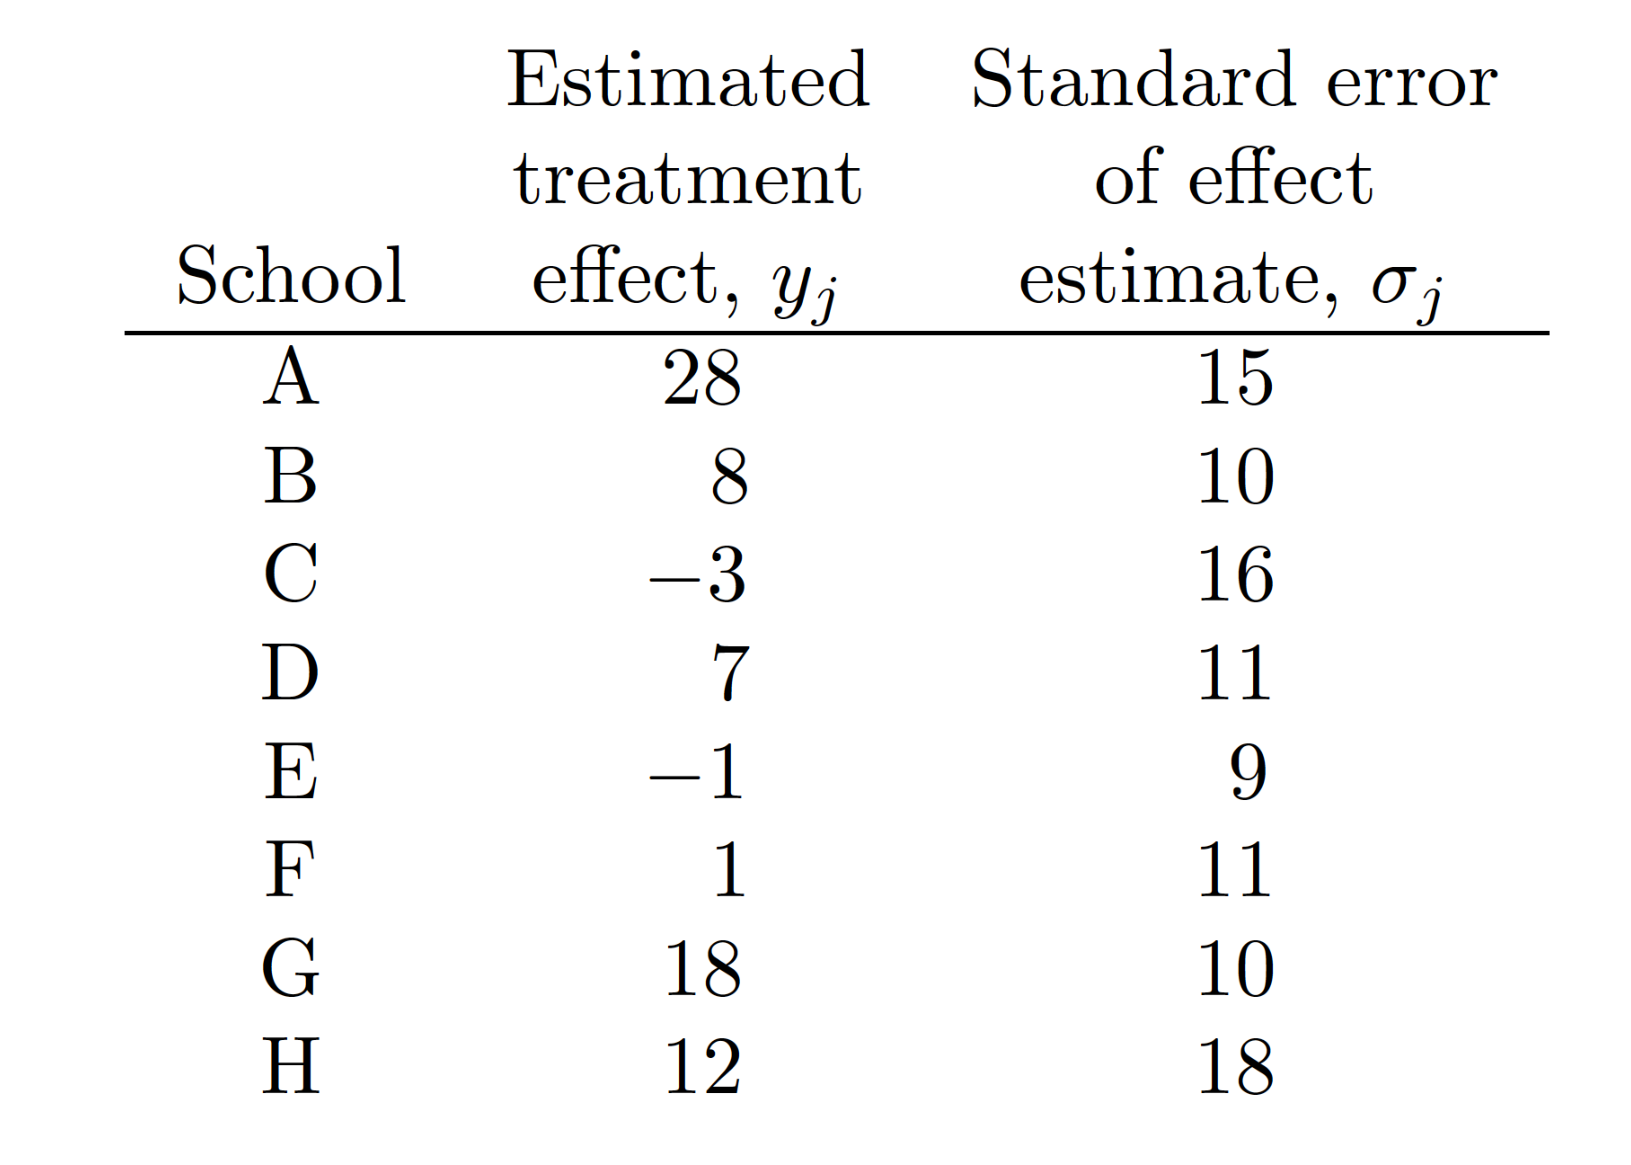
\includegraphics[width=0.5\textwidth]{8school_data.pdf}
\caption{Data for 8 schools.}
\end{figure}
Consider J experiments, each has $n_{ij}$ data points generated from normal with mean parameter $\theta_j$ and known variance $\sigma^2$:
$$y_{ij}|\theta_j \sim N(\theta_j, \sigma^2)$$
Sufficient statistic for $\theta_j$ is $\bar y_{.j}$: $$\bar y_{.j}|\theta_j \sim N(\theta_j, \sigma^2_j = \sigma^2/n_j)$$
\begin{enumerate}
\item Consider each experiment indepently. With noninformative prior, $p(\theta_j) \propto 1$, what is the posterior of $\theta_j$?
\item Consider J experiment jointly, suppose $\theta_j|\mu, \tau^2 \sim N(\mu, \tau^2),\ j \in \{1,2,..,J\}$, what is the posterior of $\theta_j$? What if $\tau^2 = 0 $ and $\tau^2 = \infty$?
\item How should we set $\mu$ and $\tau^2$? A full Bayesian approach treats $\mu$ and $\tau^2$ as unknown and having their own prior. This is called hierarchical model and $(\mu, \tau^2)$ are hyperparameters whose prior is called hyperprior. Usually we don't have much information about the hyperparameters and assign a diffuse prior distribution, i.e. $p(\mu, \tau) \propto 1$. What is the posterior distribution $p(\mu, \tau^2|y)$? 
\item In order to get posterior samples of $(\mu, \tau)$, we could rewrite the posterior as $p(\mu, \tau^2|y) = p(\mu|\tau^2, y)p(\tau^2|y)$, thus first sample $\tau^2$ from  $p(\tau^2|y)$ and then sample $\mu$ from $ p(\mu|\tau^2, y)$. What are $p(\tau^2|y)$ and $ p(\mu|\tau^2, y)$?
\end{enumerate}
\begin{figure}[!hbt]
\center
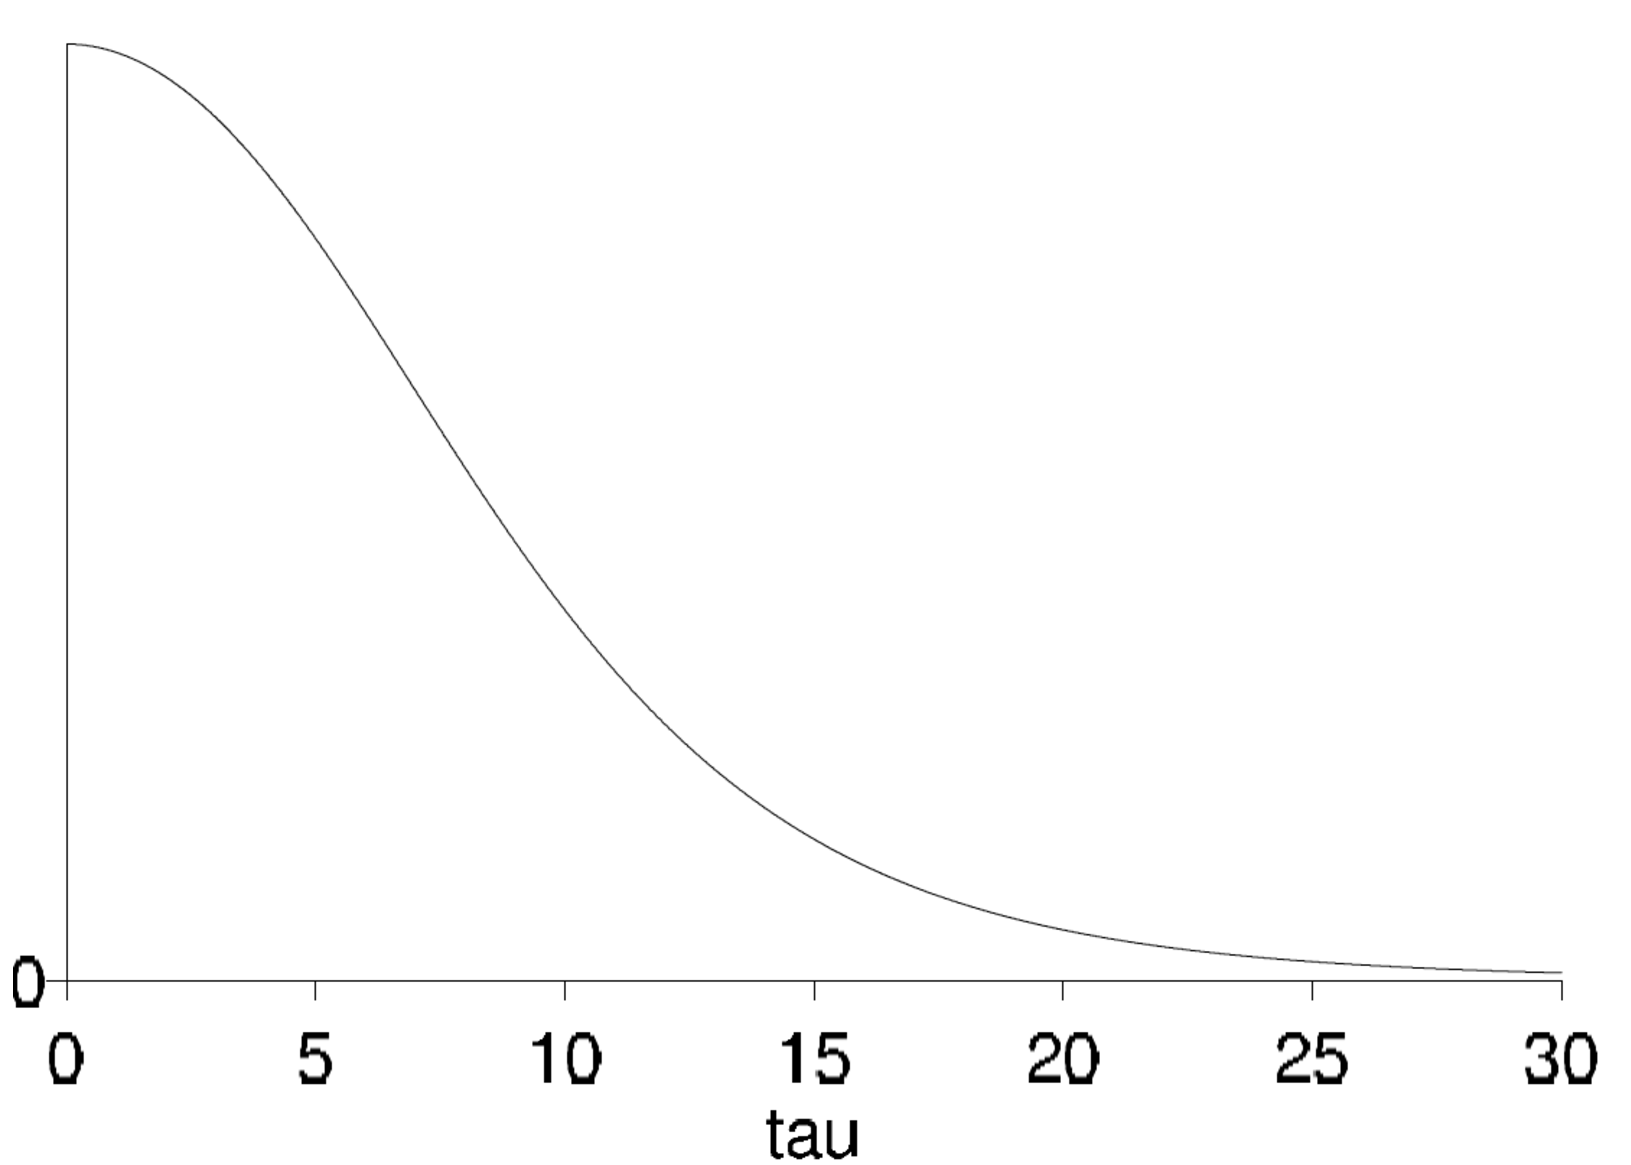
\includegraphics[width=0.5\textwidth]{8school_post_tau.pdf}
\caption{Posterior distribution $p(\tau^2|y)$.}
\end{figure}

\begin{figure}[!hbt]
\center
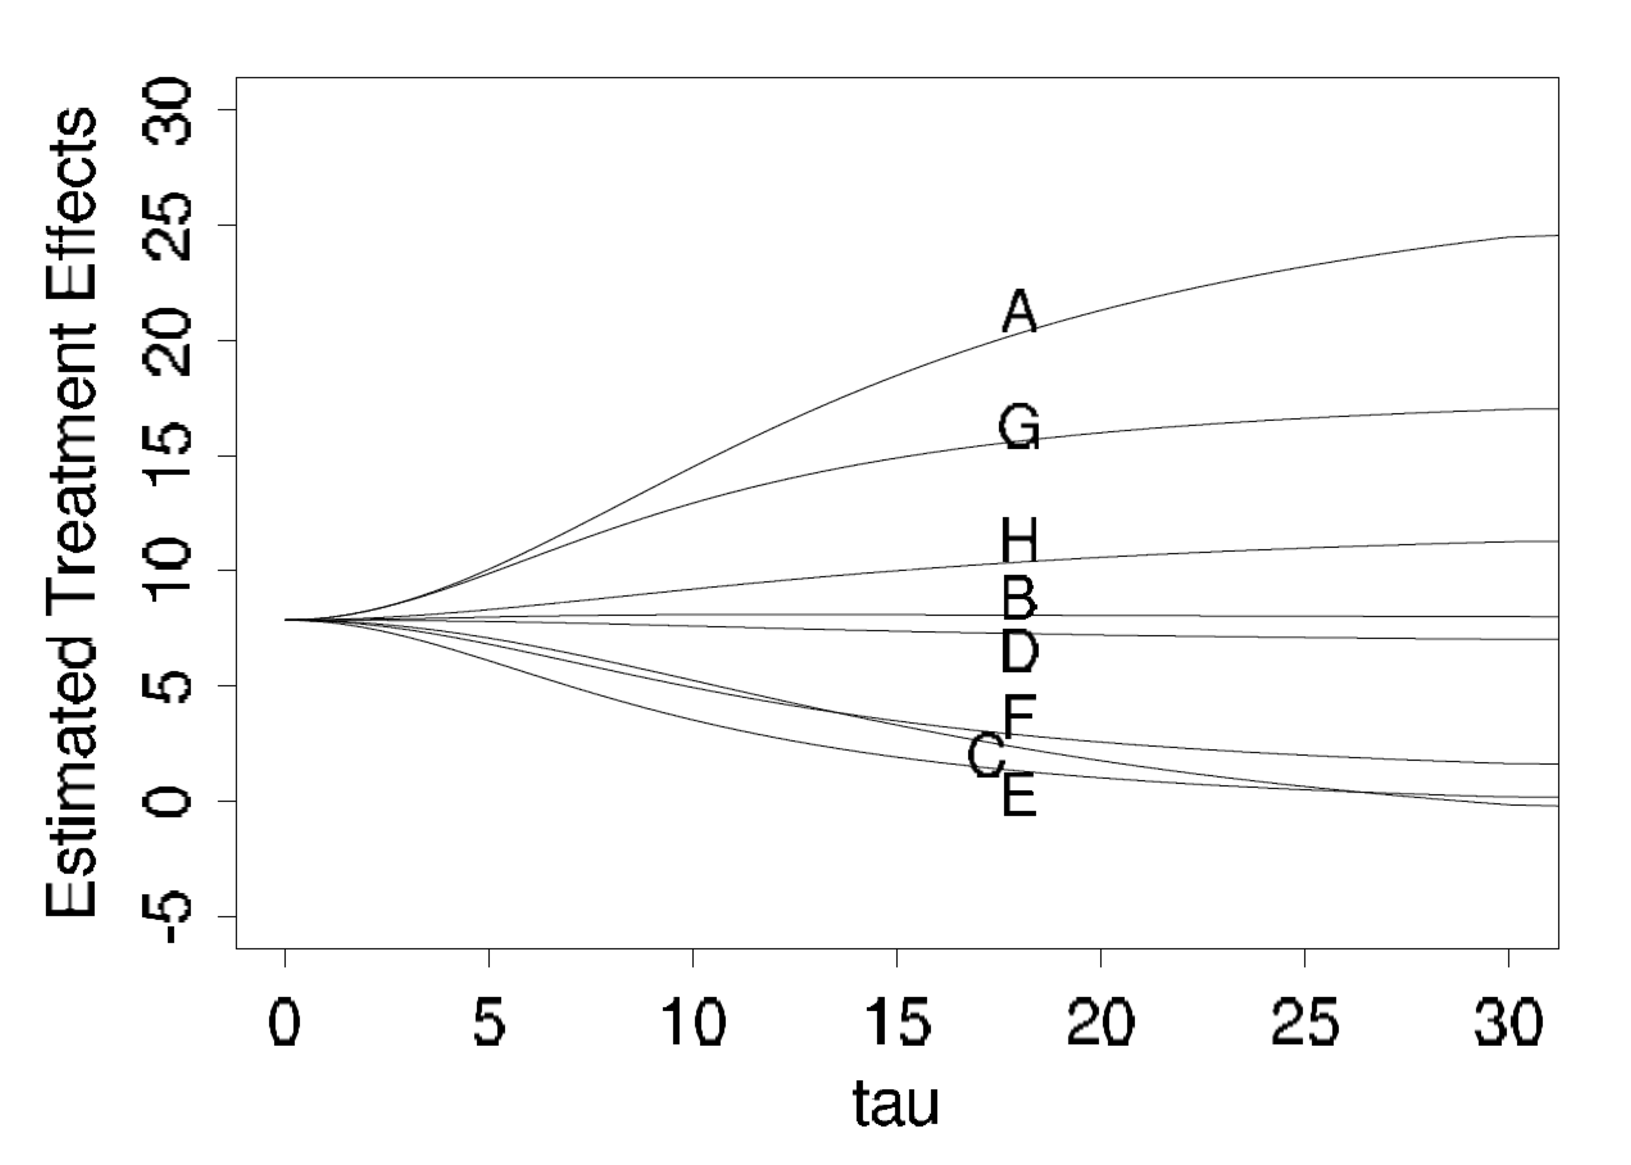
\includegraphics[width=0.45\textwidth]{8school_post_mean.pdf}
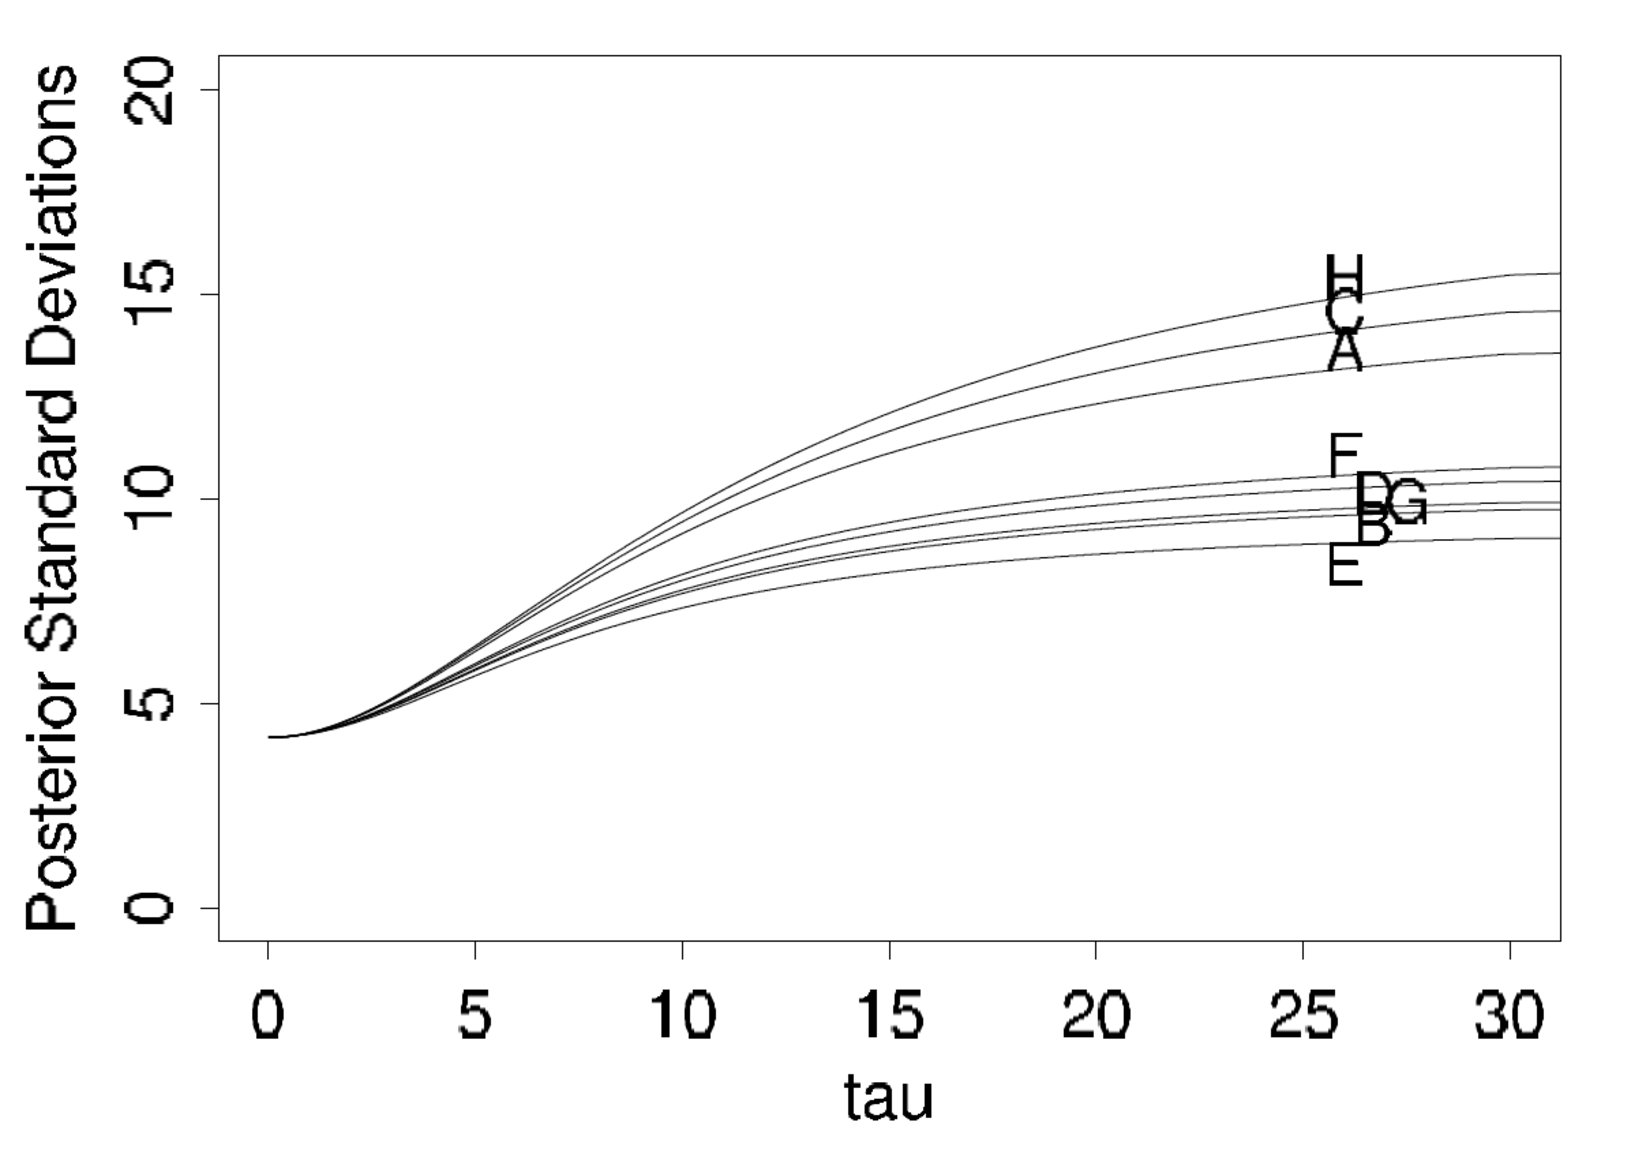
\includegraphics[width=0.45\textwidth]{8school_post_sd.pdf}
\caption{Posterior mean and standard deviation of $\theta_j$ at different values of $\tau^2$.}
\end{figure}

\begin{figure}[!hbt]
\center
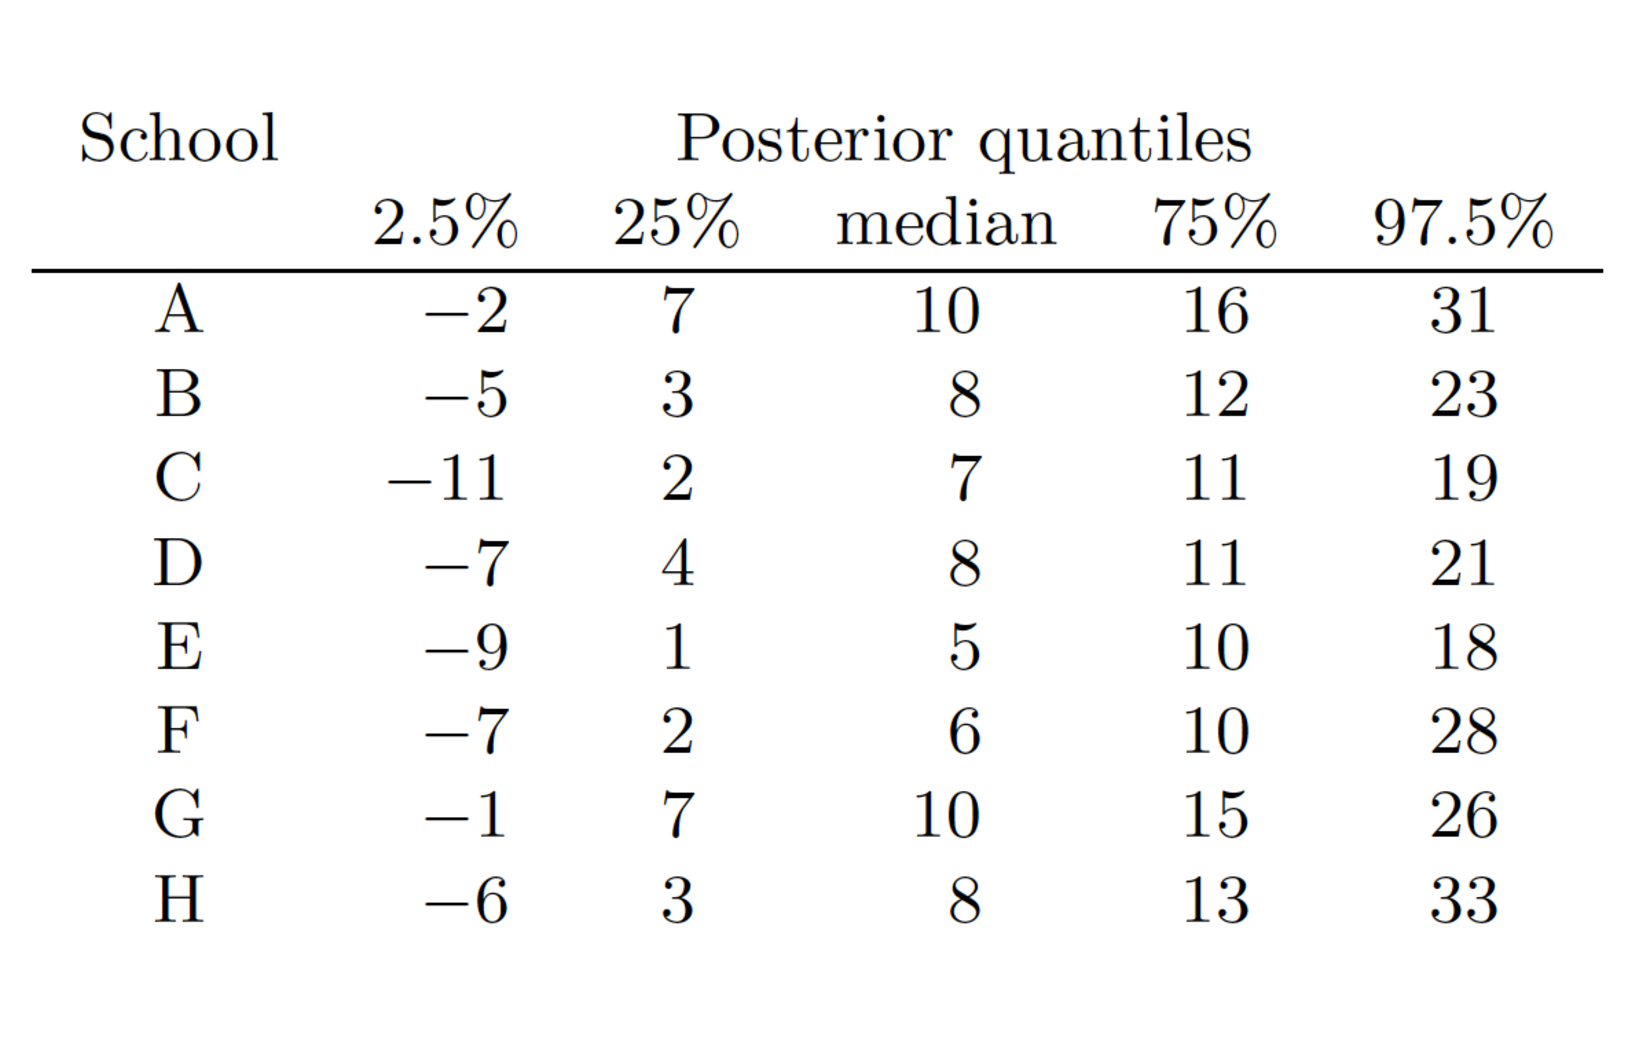
\includegraphics[width=0.5\textwidth]{8school_post_table.pdf}
\caption{Posterior distribution $p(\tau^2|y)$.}
\end{figure}

\subsection{Solution}
\begin{enumerate}
\item The posterior of $\theta_j$ is $\theta_j| y_{ij} \sim N(\bar y_{.j},  \sigma_j^2)$.
\item The posterior of $\theta_j$ is $\theta_j| y_{ij}, \mu, \tau \sim N(\frac{\frac{n_j\bar y_{.j}}{\sigma^2} + \frac{\mu}{\tau^2}}{\frac1\tau^2 + \frac{n_j}{\sigma^2}},  \frac{1}{\frac{1}{\tau^2} + \frac{n_j}{\sigma^2}})$. When $\tau^2 =0$, $\theta_j$s are equal, that is, every school has the same mean $\mu$; when $\tau^2 =\infty$, $\theta_j$s are independent and posterior of $\theta_j$ only depends on $\bar y_{.j}$.
\item Integrating out $\theta_j$, the marginal distribution of $\bar y_{.j}$ is $$\bar y_{.j}|\mu, \tau^2 \sim N(\mu, \sigma^2_j  + \tau^2)$$
Thus the marginal posterior density is $$p(\mu, \tau|y)\propto p(\mu, \tau) \prod_{j=1}^JN(\bar y_{.j}|\mu, \sigma^2_j  + \tau^2) \propto \prod_{j=1}^JN(\bar y_{.j}|\mu, \sigma^2_j  + \tau^2) $$
\item First $$\mu|\tau^2, y \sim N(\hat\mu = \frac{\sum_{j=1}^J \frac{\bar y_{.j}}{\sigma_j^2 + \tau^2}}{\sum_{j=1}^J \frac{1}{\sigma_j^2 + \tau^2}}, \hat V_{\mu}=\frac1{\sum_{j=1}^J \frac{1}{\sigma_j^2 + \tau^2}})$$
Since $p(\tau|y ) = \frac{p(\mu, \tau|y)}{p(\mu|\tau, y)}$ holds for any $\mu$, then
$$p(\tau|y ) \propto \frac{p(\tau) \prod_{j=1}^JN(\bar y_{.j}|\mu, \sigma^2_j  + \tau^2)}{N(\mu|\hat \mu, \hat V_{\mu})} = \frac{p(\tau) \prod_{j=1}^JN(\bar y_{.j}|\hat\mu, \sigma^2_j  + \tau^2)}{N(\hat\mu|\hat \mu, \hat V_{\mu})} \propto \hat V_{\mu}^{1/2}\prod_{j=1}^J(\sigma^2_j  + \tau^2)^{-1/2}e^{-\frac{(\bar y_{.j}-\hat\mu)^2}{2(\sigma^2_j  + \tau^2)}}$$
\end{enumerate}
%%%%%%%%%%%%%%%%%%%%%%%%%%%%%%%%%%%%%%%%%
%%%%%%%%%% Linear Regression %%%%%%%%%%%%
%%%%%%%%%%%%%%%%%%%%%%%%%%%%%%%%%%%%%%%%%
\section{Linear Regression}
\subsection{Review}
% Review

\noindent Recall our regression model: we are given ``fixed" inputs $\v x$,
these are used to ``predict" outputs $y$, the prediction is linear. Recall that solving for weights in linear regression corresponds to an orthogonal
projection of the known outputs $y_i$ onto the column space of $\v x$,
that is, the linear combination of $\v x$'s features that reduce the 
distance to the true $y$. For our set of parameters $\theta$:
$$ p(\v y | \v X, \v \theta) = \mathcal{N}(\v y | \v X \v w, \sigma^2 \v I) $$

\noindent where $\v w^\top \v x$ is the linear term and 
$\sigma^2$ observation noise that is considered to be known (for now).
Make sure you are comfortable switching between single data point
and whole dataset notation. Note that Murphy uses $\mathcal{D}$
(for data) and $(\v X, \v y)$ interchangeably. The log-likelihood
for $\{(\v x_i,y_i)\}_{i=1}^N$:

$$  \log p (\mathcal{D} | \v \theta) = 
    \sum_{i=1}^N \log p (y_i | \v x_i, \v \theta) = 
    -\big[\sum_{i=1}^N (y_i - \v w^\top \v x_i)^2 + \log(const) \big]
$$

\noindent Maximum Likelihood Estimate for the weights $(\v w_{MLE})$:

$$
    \argmax_w -\big[\sum_{i=1}^N (y_i - \v w^\top \v x_i)^2\big] = 
    \argmax_w -\big[(\v y - \v X \v w)^\top(\v y - \v X \v w)\big] =
    (\v X^\top \v X)^{-1}\v X^\top \v y
$$

\noindent Being Bayesian, we now put a (normal) prior over the weights $\v w$:

$$ p(\v w) = \mathcal{N}(\v w | \v m_0, \v S_0)$$

\noindent Our likelihood is:

$$ p(\v y| \v X, \v w, \sigma^2 \v I) = 
\mathcal{N}(\v y | \v X \v w, \sigma^2 \v I)$$

\noindent The posterior over the weights (which is a distribution, 
not a single point-estimate) is proportional to the product of the 
prior and the likelihood. Writing out this product and completing the square is hard, but remember that we have our closed form solutions for the parameters
of the posterior of a linear-gaussian:
\begin{align*}
    \v S_N^{-1} &= \v S_0^{-1} + \v A^\top \v \Sigma_y^{-1} \v A \\
    \v m_N &= \v S_N\big[\v S_0^{-1} \v m_0 + 
    \v A^\top \v \Sigma_y^{-1} (\v y - \v b) \big]
\end{align*}

\noindent Looks familiar. Recall the general case:

\begin{align*}
    \v x &\sim \mathcal{N}(\v m_0, \v \Sigma_0) \\
    \v y | \v x &\sim \mathcal{N}(\v A \v x + \v b, \v \Sigma_y) \\
    p(\v x | \v y) &\propto p(\v x)p(\v y | \v x) \\
    \v S_N^{-1} &= 
    \v \Sigma_0^{-1} + \v A^\top \v \Sigma_{y}^{-1} \v A \\
    \v m_N &=
    \v S_N \big[\v \Sigma_0^{-1} \v m_0 +
    \v A^\top \v \Sigma_{y}^{-1}(\v y - \v b)\big]
\end{align*}

\noindent Our case is the same with $\v b = \v 0, \v A = \v X, \v y = \v y, 
\v \Sigma_y = \sigma^2 \v I$. To connect our notation with Murphy, 
$\v m_0 = \v m_x, \v \Sigma_0 = \v \Sigma_{x}, 
\v S_N = \v \Sigma_{x|y}, \v m_N = \v m_{x|y}$.

\newpage

\noindent Returning to regression, we can now state the posterior distribution:

$$ p(\v w | \v x, \v y, ...) = 
    \mathcal{N}(\v w | \v S_N 
    \big[\v S_0^{-1} \v m_0 + \frac{1}{\sigma^2} \v X^\top \v y \big],
    \big[ \v S_0^{-1} + \frac{1}{\sigma^2}\v X^\top \v X\big]^{-1})$$

\noindent If you multiply the $\v S_N$ in the mean out, 
and replace $\v S_N$ for its definition in terms of $\v X$, 
the MLE for $\v w$ comes out as one of the terms.
Finally, the posterior predictive:

\begin{align*}
    p(\tilde{y} | \v x_{*}, \v X ,\v y) = \int 
    \mathcal{N}(\tilde{y}|\v x_{*}^\top \v w, \sigma^2)
    \mathcal{N}(\v w | \v m_N, \v S_N) d \v w &= \\
    \mathcal{N}(\tilde{y} | \v x_{*}^\top \v m_N, 
                \sigma^2 + \v x_{*}^\top \v S_0 \v x_{*})
\end{align*}

\noindent where the variance now depends on the data point to predict on 
$\v x_{*}$. This means that we can keep track of how certain (or uncertain) 
we are on new predictions based on what we saw (or didn't see) in our data.

\subsection{Unknown Observation Noise $\sigma^2$}
Following Murphy p.234, we now consider the case where the observation noise 
$\sigma^2$ is unknown:

$$ p(\v w, \sigma^2 | \mathcal{D}) $$

\noindent Our likelihood term looks the same:

$$ p( \v y | \v X, \v w, \sigma^2) = 
   \mathcal{N}(\v y | \v X \v w, \sigma^2 \v I) $$

\noindent One choice of a conjugate prior is the Normal-inverse Gaussian:

$$ p(\v w, \sigma^2) = NIG(\v w, \sigma^2 | \v w_0, \v S_0, a_0, b_0)
   = \mathcal{N}(\v w | \v w_0, \sigma^2 \v S_0) IG(\sigma^2|a_0,b_0)$$

\noindent where $a_0$ is a tail heaviness parameter and $b_0$ is an
asymmetry parameter. The posterior has the form:

\begin{align*}
    p(\v w, \sigma^2 | \mathcal{D}) &= 
    NIG(\v w, \sigma^2 | \v w_N, \v S_N, a_N, b_N)\\
    \v w_N &= \v S_N \big[\v S_0^{-1} \v w_0 + \v X^\top \v y \big]\\
    \v S_N &= \big[\v S_0^{-1} + \v X^\top \v X \big]^{-1}\\
    a_N &= a_0 + n/2\\
    b_N &= b_0 + \frac{1}{2} \big[\v w_0^\top \v S_0^{-1} \v w_0 +
                    \v y^\top \v y - \v w_N^\top \v S_N^{-1} \v w_N \big]
\end{align*}

\noindent The expressions for $\v w_N$ and $\v S_N$ are similar to 
the case where $\sigma^2$ is known. $a_N$ updates counts and $b_N$ 
is made up of $b_0$ (prior sum of squares), $\v y^\top \v y$
(empirical sum of squares), and error from the prior on $\v w$.

\noindent The marginals are:

\begin{align*}
    p(\sigma^2 | \mathcal{D}) &= IG(a_N,b_N)\\
    p(\v w | \mathcal{D}) &= \mathcal{T}(\v w_N, 
                             \frac{b_N}{a_N} \v S_N,
                             2a_N)
\end{align*}

\noindent Finally, when prediciting on $m$ new data points $\tilde{\v X}$,
the posterior predictive takes the form:

$$ p(\tilde{\v y} | \tilde{\v X}, \mathcal{D}) =
   \mathcal{T}(\tilde{\v y} | \tilde{\v X}\v w_N,
              \frac{b_N}{a_N}(\v I_m + \tilde{\v X} \v S_N \tilde{\v X}^\top),
              2a_N)$$

\noindent The variance of the distribution (middle of three parameters)
is made up of two components. The left is due to measurement noise
and the right is due to uncertainty in $\v w$. The latter term varies depending
on how similar $\tilde{\v X}$ are to $\v X$ (captured by $\v S_N$).



















\end{document}


